\documentclass[twoside,12pt]{article}

\setcounter{secnumdepth}{5}

\usepackage[nottoc,numbib]{tocbibind}

\usepackage{amsmath,amsfonts,amsthm,fullpage}
\usepackage{amsmath}
\usepackage{amssymb}
\usepackage{listings}
\setlength{\parindent}{0pt}
\usepackage{graphicx}
\usepackage{bm}
\usepackage[section]{placeins}
\usepackage{lipsum} % just for the example
\usepackage{array}

% Use the standard article template.
%
% The geometry package allows for easy page formatting.
\usepackage{geometry}
\geometry{letterpaper}
% Load up special logo commands.
\usepackage{doc}
% Package for formatting URLs.
\usepackage{url}
% Packages and definitions for graphics files.
\usepackage{epstopdf}
\DeclareGraphicsRule{.tif}{png}{.png}{`convert #1 `dirname #1`/`basename #1 .tif`.png}

\def\argmin{\operatornamewithlimits{arg\, min}}
\newcommand{\rbr}[1]{\left(#1\right)}
\newcommand{\cbr}[1]{\left\{#1\right\}}
\newcommand{\Ncal}{\mathcal{N}}
\renewcommand{\familydefault}{\sfdefault}
\newcolumntype{L}{>{\centering\arraybackslash}m{3cm}}

%
% Set the title, author, and date.
%
\title{ISyE6669, Fall 2016 - Team Project 2 Report }
\author{Ajay D'Souza (adsouza31)}
\author{
  D'Souza, Ajay\\
  \texttt{ajaydsouza@gatech.edu}
  \and
  Huestis, Sarah\\
  \texttt{shuestis3@gatech.edu }
  \and
  Li, Albert\\
  \texttt{albertli@gatech.edu}
  \and
  Yllander, Sean\\
   \texttt{syllander3@gmail.com}
}
\date{}
  
\iffalse
*------------------------------------------------------------*
  These are the instructions for the Final Report
*------------------------------------------------------------*

\fi

\begin{document}

\maketitle
\begin{center}
Project 2 Report
\end{center}

% Add an abstract.
\begin{abstract}
Project 2 Report for ISyE6669 Deterministic Optimization 
\end{abstract}
% Add various lists on new pages.
\pagebreak
\tableofcontents

\pagebreak
\listoffigures
\listoftables

% Start the paper on a new page.
\pagebreak



%
% Body text.
%
\section{Computation Experiments - Q1.4}
\label{p1}

\subsection{No Small Sub-tour Elimination Constraints - Q1.4.1}
\label{q_1_4_1}
The 48 city TSP tour with commenting out all the small Sub-tour constraints completed its run in 36.91 seconds. The number of generated Sub-Tour constraints during the course of the run was 171. The TSP had a optimal distance of 46837.9.  The TSP Tour for this formulation is plotted in figure $\eqref{g_q1_4_7_1}$ below. The results of this formulation are tabulated in table $\eqref{tab_q_1_4_6_1}$


$\\$
\subsection{1-City Sub-tour Elimination Constraint- Q1.4.2}
\label{q_1_4_2}
The 48 city TSP tour initialized with only the 1-City small sub-tour elimination constraint, completed its run in 31.68 seconds. The number of generated Sub-Tour constraints during the course of the run was 146. The TSP had a optimal distance of 50521.3 .  The TSP Tour for this formulation is plotted in figure $\eqref{g_q1_4_7_2}$ below. The results of this formulation are tabulated in table $\eqref{tab_q_1_4_6_1}$

$\\\\$
\subsection{2-City Sub-tour Elimination Constraint - Q1.4.3}
\label{q_1_4_3}
The 48 city TSP tour initialized with both the 1-City and 2-City small sub-tour elimination constraints, completed its run in 30.75 seconds. The number of generated Sub-Tour constraints during the course of the run was 51. The TSP had a optimal distance of 39829.1 .  The TSP Tour for this formulation is plotted in figure $\eqref{g_q1_4_7_3}$ below. The results of this formulation are tabulated in table $\eqref{tab_q_1_4_6_1}$

$\\\\$
\subsection{3-City Sub-tour Elimination Constraint - Q1.4.4}
\label{q_1_4_4}
The 48 city TSP tour initialized with the 1-City 2-City and 3-City small sub-tour elimination constraints, completed its run in 119.35 seconds. The number of generated Sub-Tour constraints during the course of the run was 27. The TSP had a optimal distance of 35207.9 .  The TSP Tour for this formulation is plotted in figure $\eqref{g_q1_4_7_4}$ below. The results of this formulation are tabulated in table $\eqref{tab_q_1_4_6_1}$

$\\\\$
\subsection{4-City Sub-tour Elimination Constraint - Q1.4.5}
\label{q_1_4_5}
The 48 city TSP tour initialized with the 1-City 2-City, 3-City and 4-City small sub-tour elimination constraints, completed its run in 3840.46 seconds ($\approxeq 64 Mins$). The number of generated Sub-Tour constraints during the course of the run was 33. The TSP had a optimal distance of 35868.7 .  The TSP Tour for this formulation is plotted in figure $\eqref{g_q1_4_7_5}$ below. The results of this formulation are tabulated in table $\eqref{tab_q_1_4_6_1}$

$\\\\$
\subsection{Comparing the Results for each formulation for the 48 City Tour - Q1.4.6}
\label{q_1_4_6}

Table $\eqref{tab_q_1_4_6_1}$ tabulates the results of the time taken in seconds, the number of constraints generated and the optimal tour distance for the 48 city tour for each of the formulations with different initial sub-tour constraints
\begin{table}[h]
\centering
\resizebox{\textwidth}{!}{
	\begin{tabular}{|c|c|c|c|}
		\hline
 		Formulation &  Time Taken(Secs) & No. of Generated Sub-tour Constraints & Optimal Tour Distance  \\
		\hline
		No Sub-tour Constraint & 36.91 & 171 & 46837.9  \\
		\hline
		1 City Sub-tour Constraint & 31.67 & 146 & 50521.3  \\
		\hline
		2 City Sub-tour Constraint & 30.75 & 51 & 39829.1   \\
		\hline
		3 City Sub-tour Constraint & 119.35 & 27 & 35207.9   \\
		\hline
		4 City Sub-tour Constraint & 3840.46 & 33 & 35868.7  \\
		\hline
	\end{tabular}
	}
	\caption[]{48 City Tour - Compare results from formulations with different Initial Sub-tour Constraints }
	\label{tab_q_1_4_6_1}
\end{table}


$\\\\$
\subsection{48 City TSP Tour plots - Q1.4.7}
\label{q_1_4_7}

The following are the plots of the tour generated by the various formulations for the 48 City tour.
$\\$

\begin{figure}[!htbp]
\centering
Figure $\eqref{g_q1_4_7_1}$ is the plot of the TSP of the 48 city tour with no initial Sub-tour constraints. 
 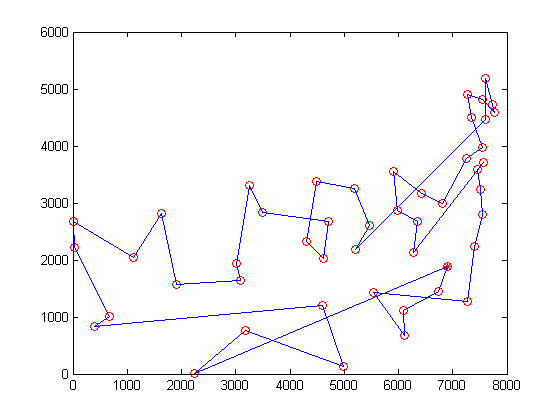
\includegraphics[scale=1.3]{0_city/all_48_with_0} 
\caption{TSP Tour Plot - 48 City Tour with no initial Sub-tour constraints}
\label{g_q1_4_7_1}
\end{figure}
\FloatBarrier


\begin{figure}[!htbp]
\centering
Figure $\eqref{g_q1_4_7_2}$ is the plot of the TSP of the 48 city tour with 1-City Sub-tour constraint. 
 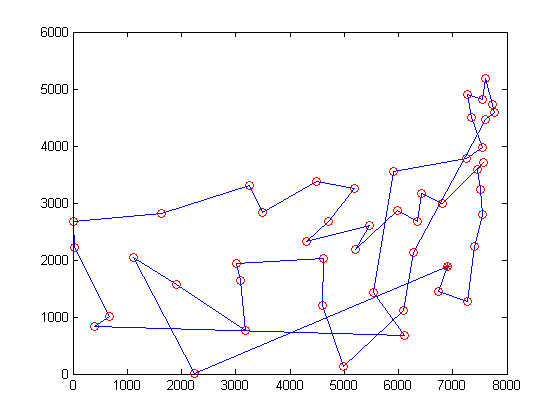
\includegraphics[scale=1.3]{1_city/all_48_with_1} 
\caption{TSP Tour Plot - 48 City Tour with 1-City initial Sub-tour constraints}
\label{g_q1_4_7_2}
\end{figure}
\FloatBarrier

\begin{figure}[!htbp]
\centering
Figure $\eqref{g_q1_4_7_3}$ is the plot of the TSP of the 48 city tour with 2-City Sub-tour constraint. 
 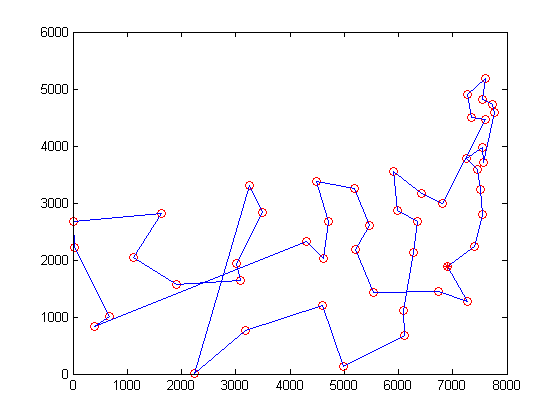
\includegraphics[scale=1.3]{2_city/all_48_with_2} 
\caption{TSP Tour Plot - 48 City Tour with 2-City initial Sub-tour constraints}
\label{g_q1_4_7_3}
\end{figure}
\FloatBarrier


\begin{figure}[!htbp]
\centering
Figure $\eqref{g_q1_4_7_4}$ is the plot of the TSP of the 48 city tour with 3-City Sub-tour constraint. 
 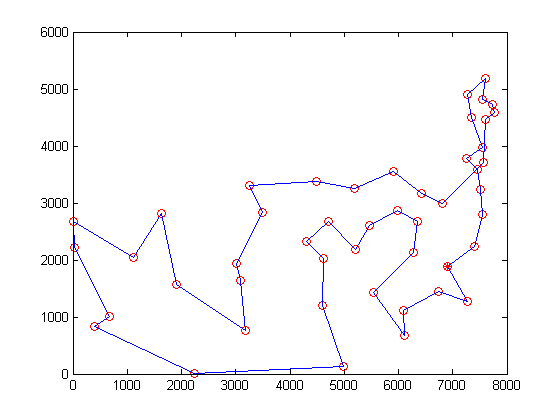
\includegraphics[scale=1.4]{3_city/all_48_with_3} 
\caption{TSP Tour Plot - 48 City Tour with 3-City initial Sub-tour constraints}
\label{g_q1_4_7_4}
\end{figure}
\FloatBarrier


\begin{figure}[!htbp]
\centering
Figure $\eqref{g_q1_4_7_5}$ is the plot of the TSP of the 48 City tour with 4-City Sub-tour constraint. 
 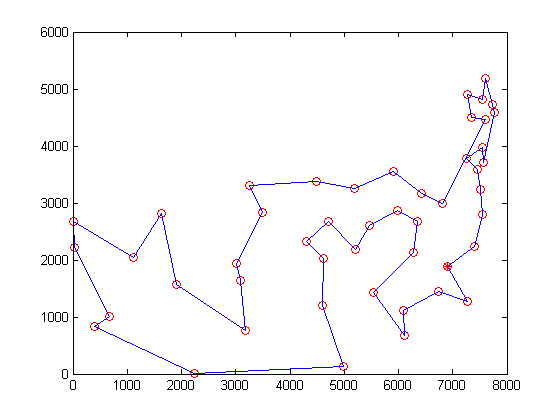
\includegraphics[scale=1.3]{4_city/all_48_with_4} 
\caption{TSP Tour Plot - 48 City Tour with 4-City initial Sub-tour constraints}
\label{g_q1_4_7_5}
\end{figure}
\FloatBarrier


$\\\\$
\subsection{48 City TSP Tour with City Names - Q1.4.8}
\label{q_1_4_8}


$\\\\$
\subsection{24 City TSP Tour - Q1.4.9}
\label{q_1_4_9}

The following are the 24 cities randomly chosen for the 24 city tour
\begin{verbatim}
coord  : [
1 6898 1885
3 5530 1424
4 401 841
5 3082 1644
6 7608 4458
8 7265 1268
11 5468 2606
15 6347 2683
16 6107 669
19 7732 4723
20 5900 3561
21 4483 3369
23 5199 2182
26 675 1006
30 7352 4506
31 7545 2801
34 4608 1198
35 23 2216
38 7392 2244
40 6271 2135
43 7280 4899
44 7509 3239
47 5185 3258
48 3023 1942]
\end{verbatim}


$\\\\$
\subsubsection{Comparing the Results for each formulation for the 24 City Tour}
\label{q_1_4_9_1}
The 24 City tour was done using the different initial small sub-tour constraints from no city to 4-City.
$\\\\\\$
Table $\eqref{tab_q_1_4_9_1}$ tabulates the results of the time taken in seconds, the number of constraints generated and the optimal tour distance for the 24 city tour for each of the formulations with different initial sub-tour constraints$\\$
\begin{table}[h]
\centering
\resizebox{\textwidth}{!}{
	\begin{tabular}{|c|c|c|c|}
		\hline
 		Formulation &  Time Taken(Secs) & No. of Generated Sub-tour Constraints & Optimal Tour Distance  \\
		\hline
		No Sub-tour Constraint & 4.56 & 72 & 33974.5  \\
		\hline
		1 City Sub-tour Constraint & 1.25 & 17 & 26876.8  \\
		\hline
		2 City Sub-tour Constraint & 1.54 & 12 & 25695.4   \\
		\hline
		3 City Sub-tour Constraint & 5.43 & 13 & 28413.2   \\
		\hline
		4 City Sub-tour Constraint & 33.35 & 5 & 25353.6  \\
		\hline
	\end{tabular}
	}
	\caption[]{24 City Tour - Compare results from formulations with the different Initial Sub-tour Constraints}
	\label{tab_q_1_4_9_1}
\end{table}

$\\\\$
\subsubsection{24 City Tour - Plotting the Results for each formulation}
\label{q_1_4_9_2}
The following figures plot the 24 City tours generated with each different small sub-tour constraints
$\\$

\begin{figure}[!htbp]
\centering
Figure $\eqref{g_q1_4_9_1}$ is the plot of the TSP of the 24 city tour with no initial Sub-tour constraints. 
 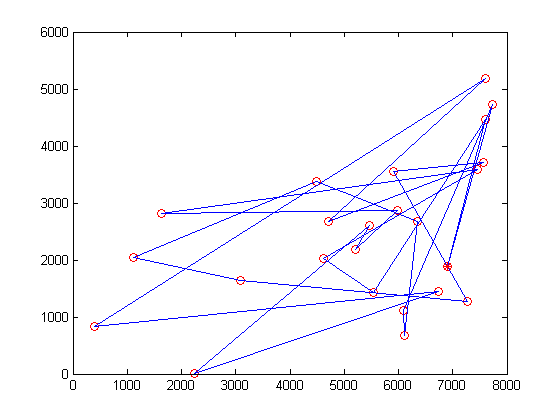
\includegraphics[scale=1.3]{0_city/all_24_with_0} 
\caption{TSP Tour Plot - 24 City Tour with no initial Sub-tour constraints}
\label{g_q1_4_9_1}
\end{figure}
\FloatBarrier


\begin{figure}[!htbp]
\centering
Figure $\eqref{g_q1_4_9_2}$ is the plot of the TSP of the 24 city tour with 1-City Sub-tour constraint. 
 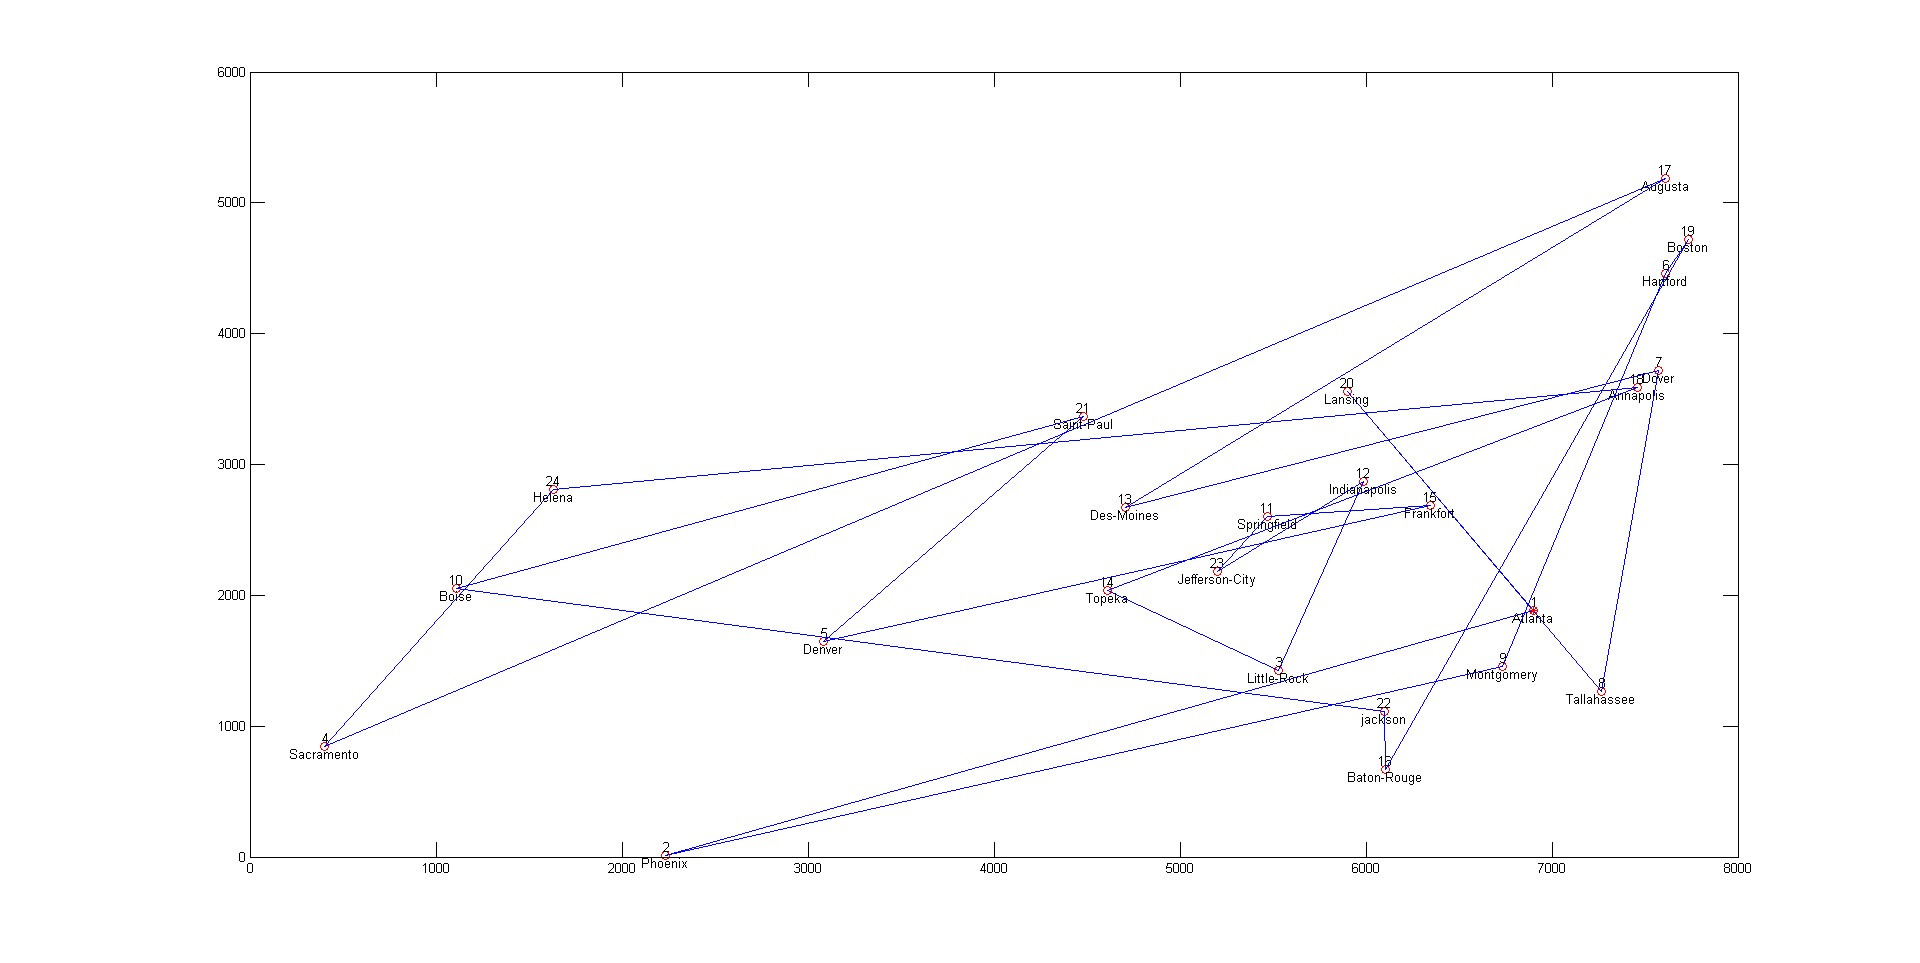
\includegraphics[scale=1.3]{1_city/all_24_with_1} 
\caption{TSP Tour Plot - 24 City Tour with 1-City initial Sub-tour constraints}
\label{g_q1_4_9_2}
\end{figure}
\FloatBarrier

\begin{figure}[!htbp]
\centering
Figure $\eqref{g_q1_4_9_3}$ is the plot of the TSP of the 24 city tour with 2-City Sub-tour constraint. 
 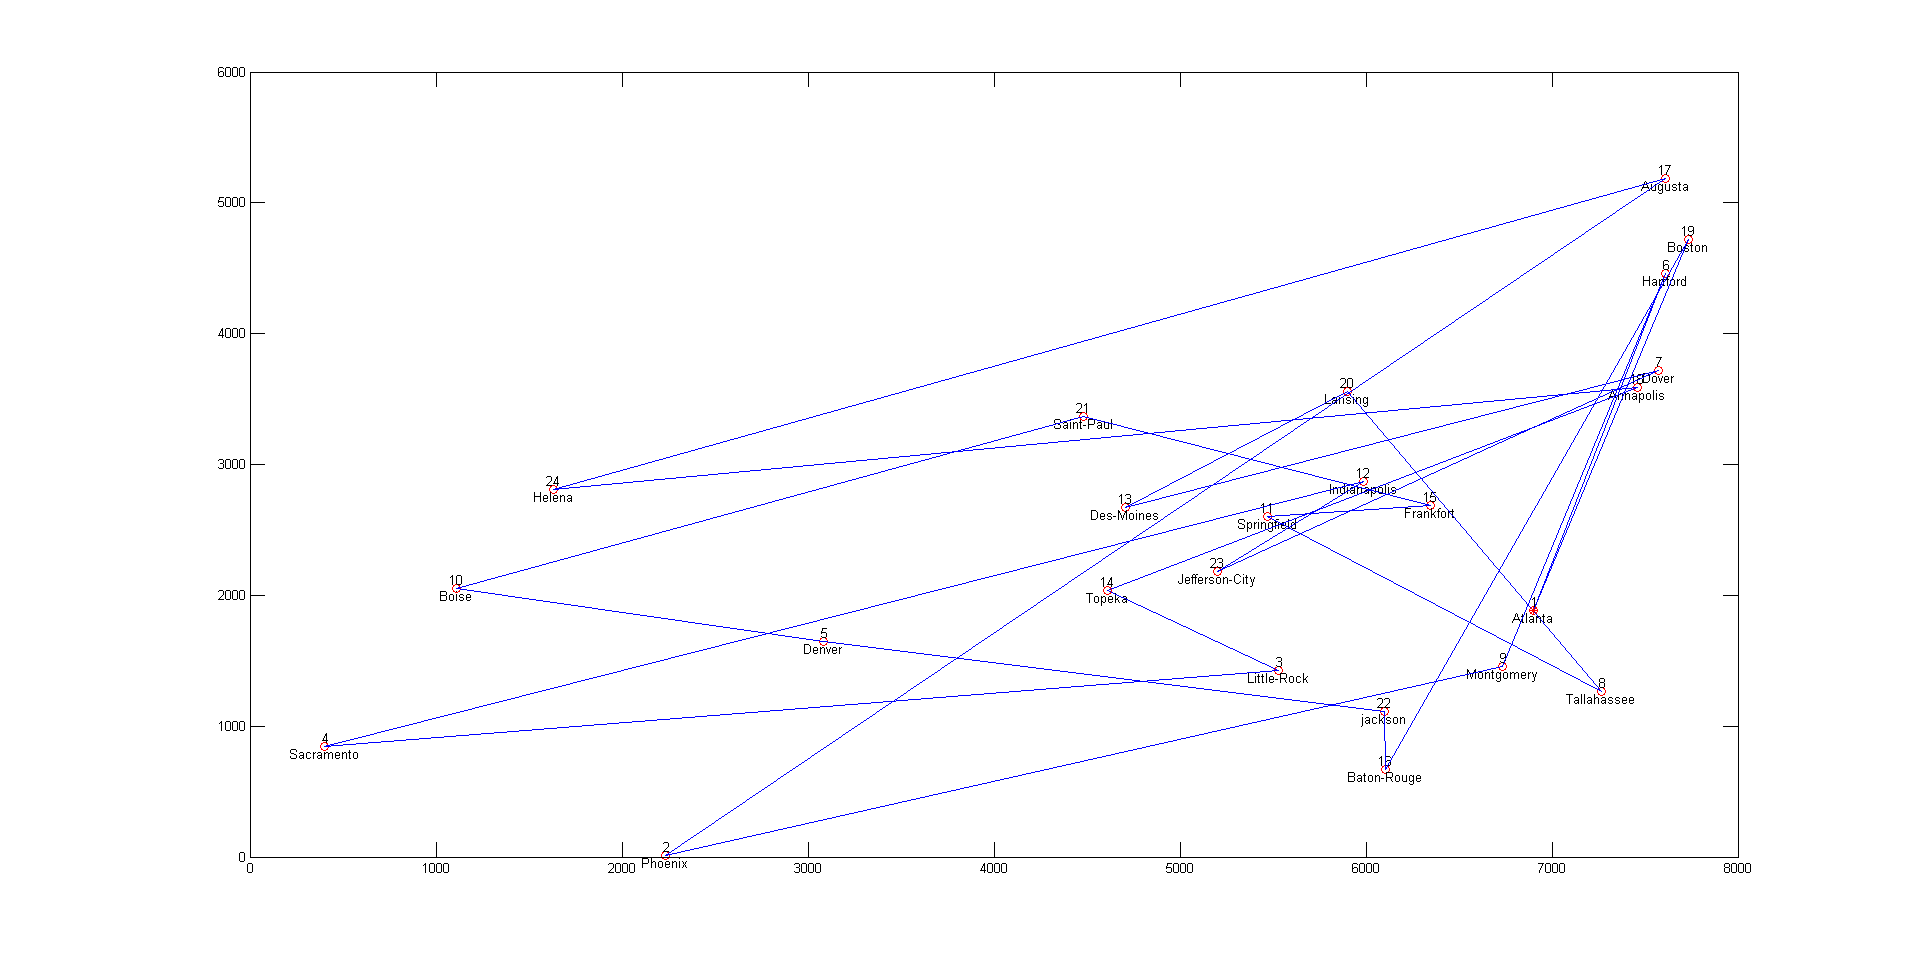
\includegraphics[scale=1.3]{2_city/all_24_with_2} 
\caption{TSP Tour Plot - 24 City Tour with 2-City initial Sub-tour constraints}
\label{g_q1_4_9_3}
\end{figure}
\FloatBarrier


\begin{figure}[!htbp]
\centering
Figure $\eqref{g_q1_4_9_4}$ is the plot of the TSP of the 24 city tour with 3-City Sub-tour constraint. 
 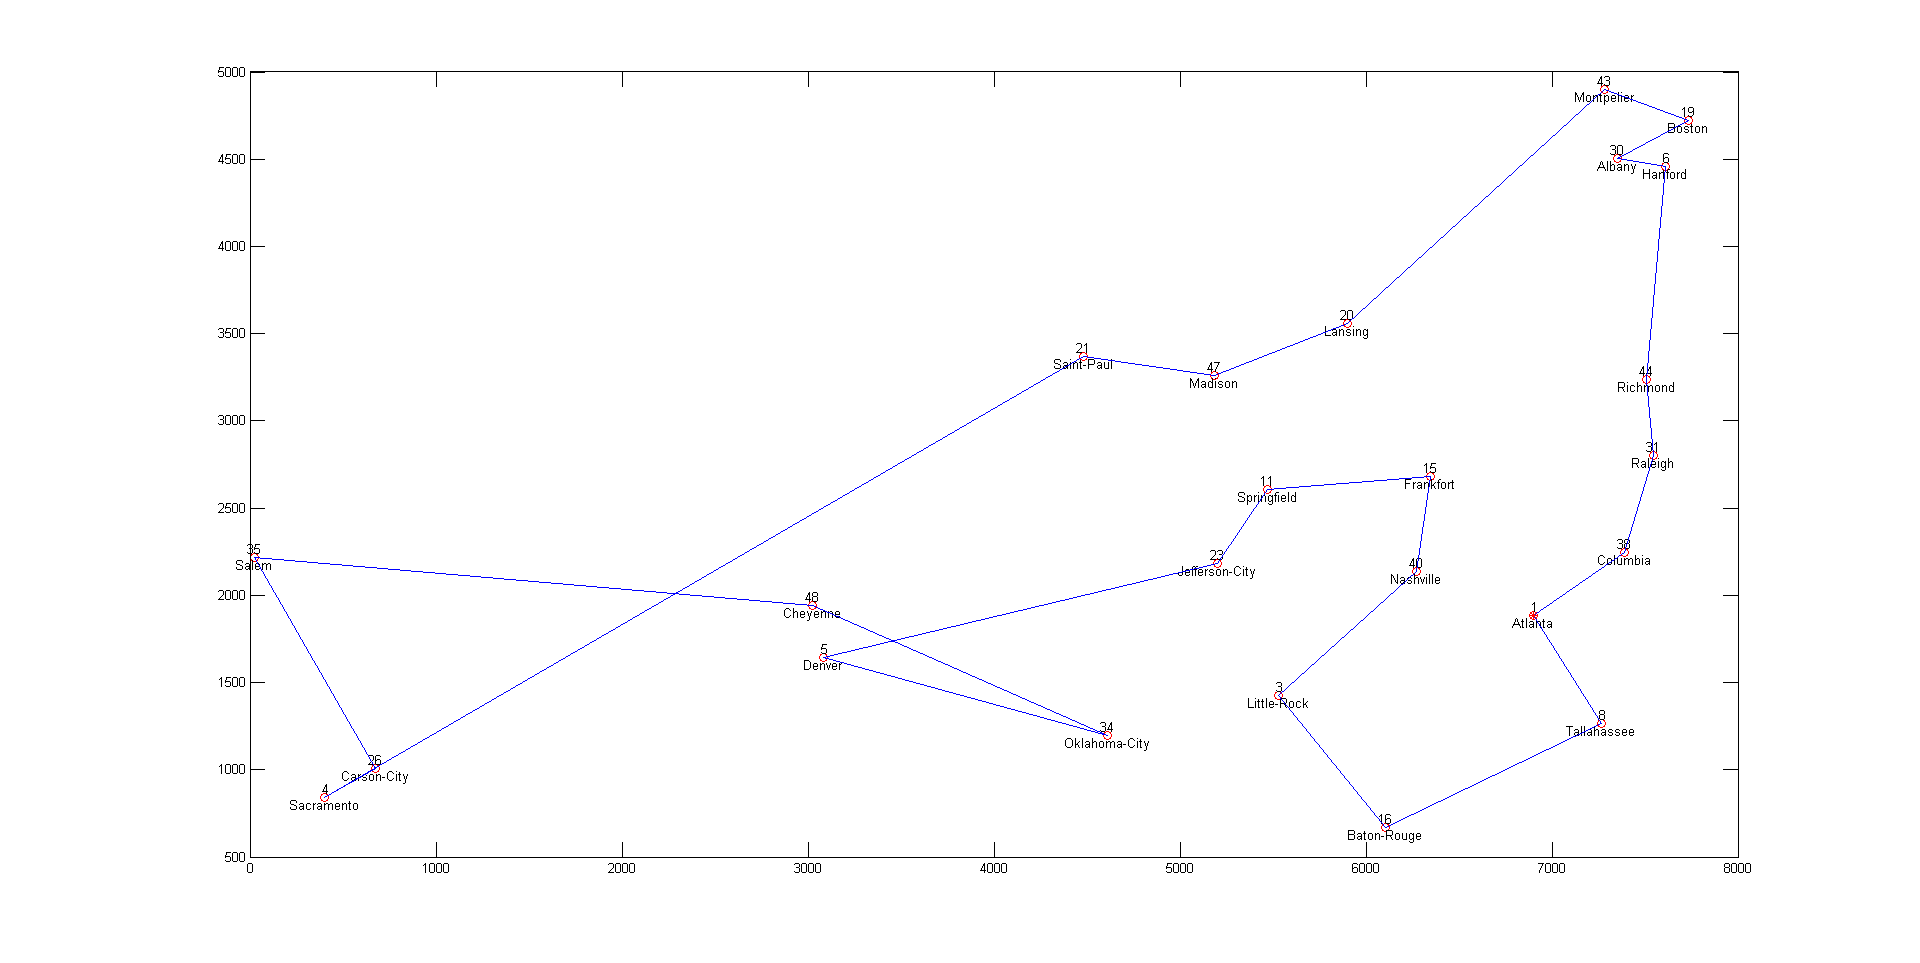
\includegraphics[scale=1.2]{3_city/all_24_with_3} 
\caption{TSP Tour Plot - 24 City Tour with 3-City initial Sub-tour constraints}
\label{g_q1_4_9_4}
\end{figure}
\FloatBarrier

$\\$
\begin{figure}[!htbp]
\centering
Figure $\eqref{g_q1_4_9_5}$ is the plot of the TSP of the 24 city tour with 4-City Sub-tour constraint. 
 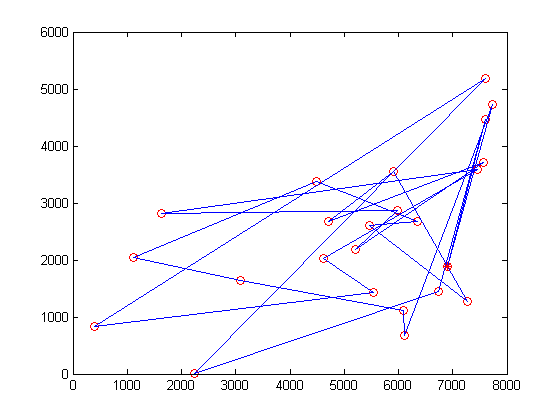
\includegraphics[scale=1.35]{4_city/all_24_with_4} 
\caption{TSP Tour Plot - 24 City Tour with 4-City initial Sub-tour constraints}
\label{g_q1_4_9_5}
\end{figure}
\FloatBarrier


$\\\\$
\section{Source Code}

The following is the source code for file $TSP-DFJ-partial.mos$ for the 48 city tour with 3-City and 4-City small sub-tour initial constraints commented out.

\subsection{TSP-DFJ-partial.mos}
\begin{verbatim}
model ModelName
uses "mmxprs"; !gain access to the Xpress-Optimizer solver
uses "mmsystem" ! include package to operating systems

N := 48  ! number of cities

declarations
	Cities = 1 .. N                         	! set of cities
	coord: array(Cities,1..3) of real			! array of coordinates of cities, to be read from US48.dat
	dist: array(Cities,Cities) of real  		! distance between each pair of cities
	x : array(Cities,Cities) of mpvar       	! decision variables
	flag : integer                          	! flag=0: not optimal yet; flag=1: optimal 
	ind : range                             	! dynamic range
	numSubtour : integer                    	! number of generated subtours
	numSubtourCities : integer					! number of cities on a generated subtour
	SubtourCities : array(Cities) of integer	! SubtourCities(i)=1 means city i is on the subtour 
	subtourCtr : dynamic array(ind) of linctr   ! dynamic array of subtour elimination constraints
	TotalDist : linctr    						! objective constraint
	
	! constraint for only one path out of each city
	leavingConstraint: array(Cities)  of linctr      
	! constraint for only one path into of each city
	enteringConstraint: array(Cities)  of linctr     
	! constraints for preventing one city subtour
	oneCitySubTourConstraint: array(Cities)  of linctr     
	! constraints for preventing two city subtour
	twoCitySubTourConstraint: dynamic array(range)  of linctr     
	! constraints for preventing three city subtour
	threeCitySubTourConstraint: dynamic array(range)  of linctr  
	! constraints for preventing four city subtour
	fourCitySubTourConstraint: dynamic array(range)  of linctr  
	
	! constraint for a TSP tour to have N edges
	!tspConstr: linctr
	
	! counter for dynamic arrays
	cons: integer          
	
	! time variables
	starttime: real
	 
	! keep track of next city for each city
	nextCity: array(Cities) of integer
	
	! keep the set of cities in the subtour, used to get the smallest subtour
	! in a aolution
	smallestSubTourSet, allSubTourCitiesSet, new_tour: set of integer
	
end-declarations

!!!!!!!!!!!!!!!!!!!!!!!!!!!!!!!!!!!!!!!!!!!!!!!!!!!!!!!!!!!!!!!!!!!!!
!!!!!  save the tour to output file for plotting !!!!!!!!!!!!!!!!!!!!
!!!!!!!!!!!!!!!!!!!!!!!!!!!!!!!!!!!!!!!!!!!!!!!!!!!!!!!!!!!!!!!!!!!!!

! record initial time
starttime:=gettime 

fopen("l_US"+N+".output",F_OUTPUT)
writeln("Starting at time :",starttime)
fclose(F_OUTPUT)

! initialization part is given 
initializations from "US"+N+".dat"
     coord
end-initializations

! compute dist(i,j) the distance between each pair of cities using (x,y) 
! coordinates of the cities, which are in the array coord
! you may need square root function sqrt()
!!!!!!!!!!!!!!! fill in your code here !!!!!!!!!!!!!!!!!!!! 
forall ( i in Cities ) do
	forall ( j in Cities ) do
		if ( i = j) then
			dist(i,j) := 0.0
		else
			dist(i,j) := sqrt( (coord(i,2)-coord(j,2))^2 + (coord(i,3)-coord(j,3))^2 )
			dist(j,i) := dist(i,j)
		end-if
	end-do
end-do

!!!!!!!!!!!!! objective: total distance of a tour
!!!!!!!!! fill in your code here !!!!!!!!!!!!!!!
TotalDist := sum(i in Cities, j in Cities ) x(i,j)*dist(i,j)

!!!!!!!!!! write constraint: x(i,j) is binary !!!!!!!!!!!!!!!!
!!!!!!!!! fill in your code here !!!!!!!!!!!!!!!
forall(i in Cities, j in Cities ) do
	x(i,j) is_binary
end-do

!!!!!!!!!!! write assignment constraints: in and out constraints for each city !!!!!!!!!!!!!!!!!!!
!!!!!!!!! fill in your code here !!!!!!!!!!!!!!!
forall(i in Cities) do
 leavingConstraint(i) := sum ( j in Cities ) x(i,j) = 1 
end-do

forall(j in Cities) do
 enteringConstraint(j) := sum ( i in Cities ) x(i,j) = 1 
end-do

! 1.
!!!!!!!!!! write 1-city subtour elimination constraints here !!!!!!!!!!!!!!!!!
!!!!!!!!! fill in your code here !!!!!!!!!!!!!!!
! generate the 48c2 combinations and add the constraint for each
! combination

forall(i in Cities) do
 ! add the no closed loop constraint for each 1 city combination
 oneCitySubTourConstraint(i) := x(i,i) = 0 
end-do


!2.
!!!!!!!!!!! write 2-city subtour elimination constraints here !!!!!!!!!!!!!!!!!!!
!!!!!!!!! fill in your code here !!!!!!!!!!!!!!!
cons := 1
! generate the 48c2 combinations and add the constraint for each
! combination
forall(i in Cities, j in Cities) do
 
 if (i>=j) then
   next
 end-if
  
 create(twoCitySubTourConstraint(cons))
 
 ! add the no closed loop constraint for each 2 city combination
 twoCitySubTourConstraint(cons) := x(i,j) + x(j,i ) <= 1
 
 cons += 1
end-do


! 3.
!!!!!!!!!! write 3-city subtour elimination constraints here !!!!!!!!!!!!!!
!!!!!!!!! fill in your code here !!!!!!!!!!!!!!!
(!
cons := 1
! generate the 48c3 combinations and add the constraint for each
! combination
forall(i in Cities, j in Cities, k in Cities ) do
 
 if (( i>=j) or ( i>=k) or (j>=k) ) then
 	next
 end-if
  
 create(threeCitySubTourConstraint(cons))
 
 ! add the no closed loop constraint for each 3 city combination
 threeCitySubTourConstraint(cons) :=  x(i,j) + x(i,k ) + x(j,k) +
 										x(j,i) + x(k,i ) + x(k,j) <= 2
 
 cons += 1
end-do

!4.
!!!!!!!!!! write 4-city subtour elimination constraints here !!!!!!!!!!!!!!
!!!!!!!!! fill in your code here !!!!!!!!!!!!!!!
cons := 1

! generate the 48c4 combinations and add the constraint for each
! combination
forall(i in Cities, j in Cities, k in Cities, l in Cities ) do
 
 if (( i>=j) or ( i>=k) or (i>=l) or (j>=k) or ( j>=l) or ( k>=l) ) then
 	next
 end-if
 
 create(fourCitySubTourConstraint(cons))
 
 ! add the no closed loop constraint for each 4 city combination
 fourCitySubTourConstraint(cons) :=  x(i,j) + x(i,k ) + x(i,l) + 
  										x(j,i) + x(k,i ) + x(l,i) + 
  										x(j,k) + x(j,l) +
  										x(k,j) + x(l,j) +
  										x(k,l) +
  										x(l,k) <= 3
  										
  cons += 1
end-do
!)

!!!!!!!!!!!!! constraint generation algorithm !!!!!!!!!!!!!!!!!!!!!!!!!!!!!!!!
numSubtour := 0   ! number of added subtour elimination constraints is zero
flag := 0 ! initalize flag to be 0, so no optimal solution has been found yet

repeat 
	
	!!!!!!!!!!!!!!! Solve the restricted master problem  !!!!!!!!!!!
	minimize(TotalDist)
	
	! Output the solution of the restricted master problem
	writeln("The restricted master problem is solved:")
	forall (i in Cities, j in Cities) do
		if abs(getsol(x(i,j))-1)<0.1 then  
		! note here we could have simply written "if getsol(x(i,j))=1 then", 
		! but I found cases where Xpress doesn't output all such x(i,j)'s. 
		! So this is a quick and ugly fix. 
		! You can use this trick in the later part when you need to check if x(i,j) is 1 or not
		! Also, feel free to develop your own solution
			writeln("x(",i,",",j,")=",getsol(x(i,j)))
		 ! save the next city information for each city in array
			next_city(i) := j
		end-if
	end-do
	
	!!!!!!!!!!!!!!!!!!!!!  find a subtour !!!!!!!!!!!!!!!!!!!!!!!!!!!!!!!!!!!!!!!!!!!!!!!!!!!!!!!!!!!!!!!!!
	! We want to find a subtour starting at city 1 (Atlanta) and ending at City 1 (such a subtour always exists!)
	! First, initialize a few things:
	numSubtourCities := 0    ! the number of cities on the subtour
	forall (i in Cities) do  ! SubtourCities(i)=1 if city i is on the subtour, initialize all entries to zero
		SubtourCities(i):=0  ! need to change entries when city i is found on the tour
	end-do
	SubtourCities(1) := 1  ! City 1 (Atlanta) is always on the subtour
		
	! Start the procedure to look for a subtour starting and ending at City 1. 
	! The basic algorithm is discussed in the hand-out
	! Note you need to update SubtourCities for cities that are on the subtour 
	! You also need to keep track of the number of cities numSubtourCities on the subtour
	!!!!!!!!! fill in your code here !!!!!!!!!!!!!!!
	
	! loop from atlanta till we reach atlanta back again
	currentCity := 1
	repeat
		! set of cities in this subtour
		smallestSubTourSet += {currentCity}
		
		! find the next city j for TSP from this city i
		currentCity := next_city(currentCity)
		numSubtourCities += 1
		SubtourCities(currentCity) := 1
				
	until ( currentCity = 1 )
	
	!!!!!!!!!!!!!!!!!!!!!!!!!!!!!!!!!!!!!!!!!!!!!!!!!!!!!!!!!!!!!!!!!!!!!!!!!!!!!!!!!!!!!!!!!!!!!!!!!!!!!!!!!
	
	! output the subtour you found
	writeln("Found a subtour of distance ", getobjval, " and ", numSubtourCities, " cities")
	writeln("Cities on the subtour are:")
	forall (i in Cities | SubtourCities(i) = 1) do
	! Note: forall ( ... | express ) is very useful, you may need to use it in the following 
	! part to add subtour elimination constraints
		write(i, " ")
	end-do
	writeln("")
	
	!!!!!!!!!!!!!!!!!!!!!!!!!!!!!!!!!!!!!!!!!!!!!!!!!!!!!!!!!!!!!!!!!!!!!
	!!!!!  save the tour to output file for plotting !!!!!!!!!!!!!!!!!!!!
	!!!!!!!!!!!!!!!!!!!!!!!!!!!!!!!!!!!!!!!!!!!!!!!!!!!!!!!!!!!!!!!!!!!!!
	fopen("l_US"+N+".output",F_OUTPUT+F_APPEND)
	writeln("Constraints Added : ",numSubtour)
	writeln("Time in Secs : ", gettime-starttime)
	writeln("Objective Distaince : ", getobjval)
	writeln("Subtour from Atlanta : ", numSubtourCities)
	writeln("Full Tour:")
	forall (i in Cities) do
		writeln(i,"\t",next_city(i))
	end-do
	writeln("--------------------------")
	fclose(F_OUTPUT)
	
	!!!!!!!!!!!!!!!!!!!! add the subtour elimination constraint !!!!!!!!!!!!!!!!!!!!!!!!!!!!!!!!!!!!!!!!!!!!!
	! If the subtour found above is indeed a subtour (i.e. has fewer than 48 cities), 
	! then add the corresponding subtour elimination
	!  constraint to the problem
	! otherwise, if the subtour has 48 cities, then it's a TSP tour and optimal, 
	! terminate the constraint generation by setting the flag to 1
	!!!!!! fill in you code !!!!!!!!!!
	
	if ( numSubtourCities = N ) then
	   flag := 1
	else

		! find the smallest subtour in the solution and a constraint to break it
			
		! only if the subtout with city 1 is > 1, else it has to be the smallest size
		if getsize(smallestSubTourSet) > 1 then
			
			! set to keep track of cities in subtours xconsidered so far,
			! initialized to the set of cities in subtour with city 1
			allSubTourCitiesSet := smallestSubTourSet
			
			! go over the cities not in subtours considered so far and find a subtour for each
			forall (i in Cities) do
			
			 ! if the city is not in the subtour considered so far, then find the subtour
			 ! having this city
			 if ( i not in allSubTourCitiesSet) then
				
				! the city is not in any subtour so far, find the subtour with this city
				new_tour := {}
				currentCity := i
				repeat
					new_tour += {currentCity}
				until ( currentCity = i ) 
				
				! add the cities in this subtour to the cities in subtour so far
				allSubTourCitiesSet += new_tour
				
				! if this tour is smaller than the earlier one  then save this as the smallest
				! subtour in this solution
				if ( getsize(new_tour) < getsize(smallestSubTourSet) ) then
					smallestSubTourSet := new_tour
				end-if
				
				! if this smallest subtour is 1 then any subtour cannot be smaller than this
				! subtour in this solution
				if ( getsize(new_tour) = 1 ) then
					smallestSubTourSet := new_tour
					break
				end-if
			 
			 end-if
			 
			end-do
			
		end-if
		
		! add a constraint to break the smallest Sub Tour found 
		numSubtour += 1
		create(subtourCtr(numSubtour))
		subtourCtr(numSubtour):= sum (i in smallestSubTourSet ) x(i, next_city(i)) <= getsize(smallestSubTourSet) - 1

	end-if

    !!!!!!!!!!!!!!!!!!!!!!!!!!!!!!!!!!!!!!!!!!!!!!!!!!!!!!!!!!!!!!!!!!!!!!!!!!!!!!!!!!!!!!!!!!!!!!!!!!!!!!!!!
  
    
until flag = 1

!!!!!!!!!!!!!!!!!!!! end of the constraint generation algorithm !!!!!!!!!!!!!!!!!!!!!!!!!

	writeln("\nOptimal TSP distance = ", getobjval)
	forall (i in Cities, j in Cities) do
		if abs(getsol(x(i,j))-1)<0.1 then
			writeln("x(",i,",",j,")=",getsol(x(i,j)))
		end-if
	end-do
	
	! write the solution to an output file 
	! then run matlab code US48TourPlot.m to plot the tour
	fopen("US"+N+".output",F_OUTPUT)
	forall (i in Cities, j in Cities) do
		if abs(getsol(x(i,j))-1)<0.1 then
			writeln(i,"\t",j)
		end-if
	end-do
	fclose(F_OUTPUT)

writeln("End running model")

end-model
\end{verbatim}


\subsection{US24TourPlot.m}

The following is the source code for $US24TourPlot.m$, for plotting the TSP for the 24 City tour.

\begin{verbatim}
clear all;

outputfile = 'US24.output';
f = fopen(outputfile,'r');
x = fscanf(f, '%d\t %d', [2, inf]);
fclose(f);
x = x';

coordfile = 'US48.input';
f = fopen(coordfile,'r');
coord = fscanf(f, '%d %f %f', [3, inf]);
fclose(f);
coord = coord';

tour = zeros(24,1);
tour(1) = 1;
fromCity = 1;
for k = 1 : 24
    tour(k+1) = x(fromCity,2);
    fromCity = x(fromCity,2);
end
figure(1);
plot(coord(tour(:,1),2),coord(tour(:,1),3),'rO');
hold on;
plot([coord(tour(:,1),2);coord(1,2)],[coord(tour(:,1),3);coord(1,3)]);
plot(coord(1,2),coord(1,3),'r*'); % the star marks Atlanta.
\end{verbatim}



\section{Distribution of Team Effort}
Equal effort by all team members. Each team member implemented the solutions independently and verified the results among the team.




%\addcontentsline{toc}{section}{References}
\bibliographystyle{plain}
% Generate the bibliography.
\begin{thebibliography}{9}

\bibitem{ekstrand_2011}
  Bertsimas Dimitris, Tsitsiklis N. John,
  \emph{Introduction to Linear Optimization},
  Athena Scientific Edition 6,
  1997.

\end{thebibliography}

\end{document}